\documentclass{article}

\usepackage[dblblindworkshop]{neurips_2026}
\workshoptitle{New in ML at NeurIPS 2026}

\usepackage[utf8]{inputenc}
\usepackage[T1]{fontenc}
\usepackage{hyperref}
\usepackage{url}
\usepackage{booktabs}
\usepackage{amsfonts}
\usepackage{nicefrac}
\usepackage{microtype}
\usepackage{xcolor}
\usepackage{amsmath,amssymb}
\usepackage{graphicx}
\usepackage{cleveref}
\usepackage{caption}
\usepackage{subcaption}
\usepackage{listings}
\usepackage{enumitem}

\hypersetup{
    colorlinks=true,
    linkcolor=black,
    citecolor=black,
    urlcolor=black
}

\captionsetup{font=small, labelfont=bf, skip=4pt}

\title{Asymptotic Dictionary Correction Discovery:\\ A Deterministic, Identifiability-Aware Framework\\
for Recovering Physical Corrections from Observational Data}

\author{%
  Anonymous Author(s) \\
  Affiliation \\
  Address \\
  \texttt{email} \\
}

\begin{document}

\maketitle

\begin{abstract}
We present \textbf{ADCD} (Asymptotic Dictionary Correction Discovery), a
deterministic framework for recovering structured corrections to known physical laws
from noisy observational data.
ADCD operates in the correction-first paradigm: given a known classical baseline,
it searches exclusively for the structured correction that vanishes at the classical limit.

The framework rests on three interlocking innovations.
\emph{First}, algebraically regularized primitive functions enforce exact
asymptotic vanishing, eliminating catastrophic cancellation that corrupts
gradient-based optimization at classical limits.
\emph{Second}, a five-dimensional (MLT$\Theta$Q) Buckingham-$\pi$ engine
automatically derives physically valid dimensionless ratio arguments,
enabling correct treatment of electromagnetic and thermodynamic variables
without manual ratio specification.
\emph{Third}, a \emph{Phenomenon-Specific Taxonomy} formalizes the Bayesian prior
inherent in domain expertise: the primitive search space is restricted
to functional families whose derivation from first principles is documented in the
physics literature, excluding physically unjustified candidates
(e.g., sinusoidal oscillations of charge) without exhaustive search.

Evaluated on three canonical physics scenarios under historical low-signal
observation windows, ADCD demonstrates distinct epistemic behaviors.
For Screened Coulomb ($\Delta\mathrm{BIC} = 30.65$) and Entropy Expansion
($\Delta\mathrm{BIC} = 14.58$), the system achieves full four-step validation
(IDENTIFIABLE), with the Screened Coulomb result constituting an \emph{exact}
symbolic match whose blind provenance is certified by an internal parameter
index offset ($\theta_4$ rather than $\theta_0$).
For Time Dilation at $v \le 0.3c$, the Lorentz structure is recovered at Rank~1
but the positive control fails because the historical signal is too weak
(${\le}\,4.8\%$ correction against $1\%$ noise): the system autonomously
withholds the structural claim (WITHHELD).
This self-aware epistemic restraint is a core design property: ADCD is
engineered to report ``the data do not yet support a claim'' rather than
return a confident but unreliable answer.
All results are byte-exact deterministic across independent runs.

\vspace{0.3em}
\noindent\textbf{Keywords:} symbolic regression; correction discovery;
dimensional analysis; Bayesian prior; model selection; identifiability
\end{abstract}

% ---------------------------------------------------------------
\section{Introduction}
% ---------------------------------------------------------------

Physical laws often follow a correction-first structure: a known classical
baseline is extended by a term that vanishes at the classical
limit~\cite{einstein1905,debye1923,callen1985}.
Recovering that correction from observational data is a problem distinct from
full equation discovery: the baseline is fixed, only the residual must be found,
and the residual must vanish exactly at the boundary where classical physics holds.

General-purpose symbolic regression (SR) engines such as PySR~\cite{cranmer2023},
AI Feynman~\cite{udrescu2020}, and PhySO~\cite{tenachi2023} excel at discovering
equations from scratch, but face a cluster of difficulties in this correction-first
setting.
\emph{Catastrophic cancellation}: as the dimensionless ratio $u\to0$ and the
correction $\Delta\to0$, naive forms (e.g., $e^{-u}-1$ computed as $1-1$)
lose all significant digits to floating-point cancellation~\cite{ieee754},
causing the optimizer to receive misleading feedback precisely where the physics
is most constrained.
\emph{Stochastic irreproducibility}: evolutionary and Monte Carlo search
engines~\cite{bongard2007,schmidt2009} cannot guarantee byte-identical results
across runs, complicating audit and replication.
\emph{Silent overclaiming}: major SR engines return a single best-fit equation
regardless of whether the data carry sufficient statistical power to distinguish
among competing structures~\cite{lacava2021}.

We present ADCD, a correction-first framework designed to address all three
failure modes simultaneously.
Its algebraically regularized primitives make exact asymptotic vanishing an
algebraic identity rather than a numerical approximation.
Its deterministic grammar enumeration guarantees reproducible, auditable search.
Its four-step validation protocol uses BIC-based Ablation Control to explicitly
distinguish identifiable from unidentifiable structural claims,
reporting WITHHELD when data are insufficient rather than overclaiming.

The central question motivating ADCD is not ``can a machine rediscover known
corrections?'' but rather: ``under what data conditions can a machine
\emph{reliably} distinguish the true correction from structurally similar
alternatives, and when must it honestly refuse?''

% ---------------------------------------------------------------
\section{Related Work}
% ---------------------------------------------------------------

General SR engines (Eureqa~\cite{schmidt2009}, PySR~\cite{cranmer2023},
AI Feynman~\cite{udrescu2020,udrescu2020b}, PhySO~\cite{tenachi2023})
target unconstrained equation recovery and do not enforce classical-limit
constraints algebraically.
SINDy~\cite{brunton2016} shares our library-based approach but discovers
governing equations rather than corrections.
PINNs~\cite{raissi2019,karniadakis2021} embed physical laws as soft loss penalties;
ADCD imposes them as hard algebraic identities before any numerical computation.
AI-Descartes~\cite{cornelio2023} combines SR with axiomatic theory derivation,
but does not address catastrophic cancellation or provide identifiability gating.
While dimensional analysis has been integrated into SR~\cite{tenachi2023,petersen2021},
ADCD extends this with a full five-dimensional (MLT$\Theta$Q) Buckingham-$\pi$ engine,
transcendental argument safety, and BIC-based identifiability reporting
in a single pre-fitting gate cascade.
To our knowledge, ADCD is the first framework to combine deterministic grammar
enumeration, algebraic classical-limit enforcement, phenomenon-specific Bayesian
priors, and explicit identifiability gating for the correction-first paradigm.

% ---------------------------------------------------------------
\section{Methods}
% ---------------------------------------------------------------

\subsection{Problem formulation}

Let $y_\mathrm{obs}$ be the observed target and $y_\mathrm{cl}$ the known
classical prediction. Define the correction residual:
\begin{equation}
  \Delta =
  \begin{cases}
    y_\mathrm{obs}/y_\mathrm{cl} - 1 & \text{(multiplicative)} \\
    y_\mathrm{obs} - y_\mathrm{cl}   & \text{(additive)}
  \end{cases}
\end{equation}
The multiplicative formulation is adopted when its residual shows weaker
Spearman rank correlation with the classical prediction magnitude than the
additive residual, using a confidence-gated decision boundary that defaults
to additive mode under high ambiguity.
ADCD searches for $\hat{\Delta}(\mathbf{x};\boldsymbol{\theta})$, where
$\mathbf{x}$ is the vector of physical inputs, $\boldsymbol{\theta}$ are
continuous free parameters, and $\hat{\Delta} \to 0$ as the relevant
dimensionless ratio $u \to 0$.

\subsection{Algebraically regularized primitive dictionary}

Each primitive $D(u)$ satisfies $\lim_{u\to 0} D(u) = 0$ as an exact algebraic
identity. This eliminates catastrophic cancellation: the correction vanishes
algebraically, without subtracting large nearly-equal floating-point terms.

Table~\ref{tab:primitives} lists the five primitives.
To illustrate the precision advantage: for \texttt{D\_lor} in \texttt{float64},
the naive form $(1-u)^{-1/2}-1$ collapses to $0.0$ at $u=10^{-16}$
(all significant digits lost to cancellation); the regularized algebraic form
$u/[\sqrt{1-u}(\sqrt{1-u}+1)]$ returns $5.0\times10^{-17}$ at the same $u$.

\begin{table}[ht]
\small
\caption{The five algebraically regularized primitives, each satisfying
$\lim_{u\to0}D(u)=0$ as an exact algebraic identity.
Column ``Physical origin'' cites the fundamental equation that produces this
functional family; it does not imply the primitive is restricted to that domain.}
\label{tab:primitives}
\centering
\begin{tabular}{@{}lllp{3.5cm}@{}}
\toprule
Name & Regularized form $D(u)$ & Domain & Physical origin \\
\midrule
\texttt{D\_lor}      & $u/[\sqrt{1-u}(\sqrt{1-u}+1)]$ & $u\in[0,1)$ & Lorentz factor ($\gamma-1$) \\
\texttt{D\_rat}      & $u/(1-u)$                       & $u\neq 1$   & Yukawa/Fermi pole \\
\texttt{D\_exp}      & $e^{-u}-1$                      & all $u$     & Debye/Yukawa screening \\
\texttt{D\_log}      & $\ln(1+u)$                      & $u>-1$      & Entropy of mixing \\
\texttt{D\_sqrt\_inv}& $1/\sqrt{1+u}-1$                & $u>-1$      & Gravitational/Coulomb potential \\
\bottomrule
\end{tabular}
\end{table}

\subsection{Five-dimensional Buckingham-$\pi$ ratio generation}
\label{sec:buckingham}

ADCD employs a five-dimensional (MLT$\Theta$Q) Buckingham-$\pi$ engine
where each variable is represented as a five-vector $\mathbf{d}\in\mathbb{Z}^5$
over the SI base dimensions Mass~(M), Length~(L), Time~(T), Temperature~($\Theta$),
and Electric Charge~(Q).
The engine constructs dimensionless $\pi$-groups by computing the rational nullspace
of the dimension matrix and enumerating integer-exponent products thereof.

The extension from the conventional MLT to MLT$\Theta$Q is crucial for
correctness, not merely completeness.
In a 3D (MLT) engine, charges $q_1$ and $q_2$ carry no dimension and are
trivially treated as scalars; the engine would form $r/\theta$ as the primary
candidate ratio involving a length scale.
In the 5D engine, charges carry genuine Charge dimension~(Q); the engine must
enumerate and account for Q in every ratio candidate it generates.
This increases the number of systematically explored ratio candidates,
and the distance ratio $r/\theta$ is reached only after charge-dimensional
candidates are enumerated in order.

This enumeration order is reflected directly in the validation output.
The blind search for Screened Coulomb recovers $\theta_0(e^{-r/\theta_4}-1)$,
where subscript $4$ indicates that four ratio candidates were enumerated before
the distance-ratio argument $r/\theta_4$ was reached.
Had the ratio $r/\theta$ been supplied manually (bypassing the Buckingham-$\pi$
engine), the parameter would universally carry subscript $0$.
The non-zero subscript is therefore machine-verifiable evidence that the
dimensionless argument was derived blindly from dimensional algebra, not
from prior knowledge of the answer.

\subsection{Phenomenon-specific taxonomy as Bayesian prior}
\label{sec:taxonomy}

Each physics phenomenon is associated with a named set of permitted primitive
families, derived exclusively from the fundamental equations of that phenomenon.
For example, the taxonomy entry \texttt{yukawa\_debye\_screening} permits only
\texttt{D\_exp} and \texttt{D\_rat}, because the Klein-Gordon equation
yields $V(r)\propto e^{-mr}/r$ and Debye-H\"{u}ckel theory yields
$\phi(r)\propto e^{-r/\lambda_D}/r$: both involve only exponential and rational
functional families.
Trigonometric and power-law families are excluded because no peer-reviewed
derivation of Yukawa or Debye screening produces them.

\textbf{What the taxonomy specifies.}
The taxonomy restricts \emph{which functional family} is admitted to the
search space. It supplies nothing about \emph{which variable} enters the
dimensionless argument or \emph{what the scale parameter} is.
These are determined entirely by the Buckingham-$\pi$ engine
(Section~\ref{sec:buckingham}) and the numerical optimizer operating on data.

\textbf{What this means in practice.}
A physicist confronting a plasma shielding anomaly does not try sinusoidal
oscillations of electric charge as candidate corrections: the Debye-H\"{u}ckel
derivation rules them out.
ADCD formalizes this prior explicitly, making it documented, auditable, and
reproducible.
Including a physically unjustified primitive (such as a power-law family
not present in our dictionary) in a Yukawa scenario causes it to act as a
``noise sponge,'' absorbing variance from the distance variable and collapsing
the Ablation Control BIC gap, degrading identifiability without improving
physical interpretability.
The Phenomenon-Specific Taxonomy is not a shortcut; it is the removal of
hypotheses that the founding physics literature has already falsified.

Table~\ref{tab:taxonomy} lists the taxonomy entries for our three experiments.

\begin{table}[ht]
\small
\caption{Phenomenon-specific taxonomy entries used in experiments,
with physical justification for the primitive set.}
\label{tab:taxonomy}
\centering
\begin{tabular}{@{}p{3.8cm}p{2.4cm}p{5.4cm}@{}}
\toprule
Phenomenon key & Primitives & Justification \\
\midrule
\texttt{yukawa\_debye\_screening} & \texttt{D\_exp}, \texttt{D\_rat} &
  Klein-Gordon / Debye-H\"{u}ckel: fundamental form is $e^{-mr}/r$. \\
\texttt{lorentz\_special\_relativity} & \texttt{D\_lor} &
  Lorentz invariance of Maxwell equations uniquely selects the $\gamma-1$ form. \\
\texttt{boltzmann\_thermodynamics} & \texttt{D\_exp}, \texttt{D\_log} &
  Boltzmann partition function and entropy of mixing involve $e^{-\beta\epsilon}$ and $\ln$. \\
\bottomrule
\end{tabular}
\end{table}

\subsection{Grammar enumeration and theta-intact constraint}

Candidates take the form $\hat{\Delta}=\theta_0\cdot D_i(u_{ij})$,
optionally extended with a secondary additive correction term
(composition budget: depth up to three nested primitives).
Dimensionless arguments $u_{ij}$ are auto-generated by the Buckingham-$\pi$
engine with a budget of up to 12 candidate ratios per scenario,
ensuring sufficient coverage when multiple dimensional families (e.g., Charge and
Length) are present simultaneously.

All structural gates (Section~\ref{sec:gates}) are evaluated on the
\emph{theta-intact} expression---the fully parameterized symbolic form
before any $\theta_i$ are assigned specific numerical values.
Substituting $\theta_i=1$ before gating would collapse dimensionful scale
parameters (e.g., the ratio $r/\theta_1$ representing a Debye length)
into dimensionless constants, falsifying the dimensional consistency check.

\subsection{Physical gate cascade}
\label{sec:gates}

Before any numerical fitting, each candidate must pass a five-gate cascade
(Table~\ref{tab:gates}) applied to the theta-intact expression.

\begin{table}[ht]
\small
\caption{The five-gate pre-fitting physical cascade.}
\label{tab:gates}
\centering
\begin{tabular}{@{}p{3.5cm}p{9cm}@{}}
\toprule
Gate & Rejection criterion \\
\midrule
1. AST complexity & SymPy tree depth $>12$ or token count $>50$. \\
2. Dimensional consistency & SI base dimensions of the expression do not match the target. \\
3. Transcendental safety & Arguments to $\exp$, $\ln$, $\sqrt{\cdot}$ are not dimensionless. \\
4. Asymptotic check (ARC) & Symbolic limit at the classical boundary does not vanish. \\
5. Coarse numerical fitness & Evaluation at $\boldsymbol{\theta}=\mathbf{1}$ produces \texttt{NaN}/\texttt{Inf}. \\
\bottomrule
\end{tabular}
\end{table}

Gate~3 (Transcendental Safety) rejects expressions such as $\exp(q/\theta)$
when $q$ carries dimension Q (Electric Charge), because the argument $q/\theta$
is not dimensionless unless $\theta$ carries dimension Q as well.
This prevents dimensionally inconsistent forms from reaching the optimizer,
even when the optimizer could numerically fit them to acceptable values.

\subsection{Parameter optimization and model selection}

Surviving candidates are optimized via L-BFGS-B using JAX with
\texttt{float64} precision.
All free parameters are log-parameterized ($\theta_i = s_i e^{u_i}$,
$s_i \in \{-1,+1\}$) to allow traversal across orders of magnitude with
smooth gradients.
Multiple restarts with diverse initializations reduce sensitivity to
local optima.

Model selection uses the Bayesian Information Criterion~\cite{schwarz1978}:
\begin{equation}
  \mathrm{BIC} = k\ln N - 2\ln\hat{L}
\end{equation}
where $k$ is the number of free parameters, $N$ the data size, and $\hat{L}$
the maximized likelihood under Gaussian noise.
By the Kass--Raftery scale~\cite{kass1995}, $\Delta\mathrm{BIC}>10$
constitutes very strong evidence; we adopt this as the minimum threshold for
any identifiability claim.

\subsection{Four-step validation protocol}
\label{sec:protocol}

A structural discovery claim is made only when all four checks pass:
\begin{enumerate}[noitemsep,leftmargin=*]
  \item \textbf{Budget disclosure.} Full search space size $|\mathcal{C}|$
        and primitive list are reported before results are seen.
  \item \textbf{Positive control.} Restricted to only the ground-truth
        primitive family, the system must recover the correct structure.
  \item \textbf{Ablation control.} With the ground-truth primitive family excluded,
        the BIC gap between the correct structure and the best alternative
        must satisfy $\Delta\mathrm{BIC}>10$.
  \item \textbf{Determinism check.} Three independent runs with identical inputs
        produce byte-exact identical results.
\end{enumerate}
Failure of any single check yields WITHHELD.
Passing all four yields IDENTIFIABLE.

% ---------------------------------------------------------------
\section{Experiments}
% ---------------------------------------------------------------

\subsection{Setup}

Table~\ref{tab:scenarios} summarizes the three scenarios.
Observation windows are chosen to reflect historical low-signal regimes where
the anomalous correction was just beginning to emerge above the noise floor.
Synthetic observations use 1\% Gaussian multiplicative noise,
$N=200$ points, seed~42.
The ground truth is never provided to the pipeline at any stage;
only noisy observations, classical predictions, dimensional variable definitions,
and the taxonomy key are supplied.

\begin{table}[ht]
\small
\caption{Experimental scenarios with domains, historical observation windows,
taxonomy keys, and target primitive families.}
\label{tab:scenarios}
\centering
\begin{tabular}{@{}lllll@{}}
\toprule
Scenario & Domain & Window & Taxonomy key & Target \\
\midrule
Time Dilation     & Relativity      & $v\le0.3c$       &
  \texttt{lorentz\_special\_relativity} & \texttt{D\_lor} \\
Screened Coulomb  & Electrostatics  & $r\le4.0$~m      &
  \texttt{yukawa\_debye\_screening}     & \texttt{D\_exp} \\
Entropy Expansion & Thermodynamics  & $dV/V_i\le1.0$   &
  \texttt{boltzmann\_thermodynamics}   & \texttt{D\_log} \\
\bottomrule
\end{tabular}
\end{table}

\subsection{Results}
\label{sec:results}

\begin{figure*}[t]
  \centering
  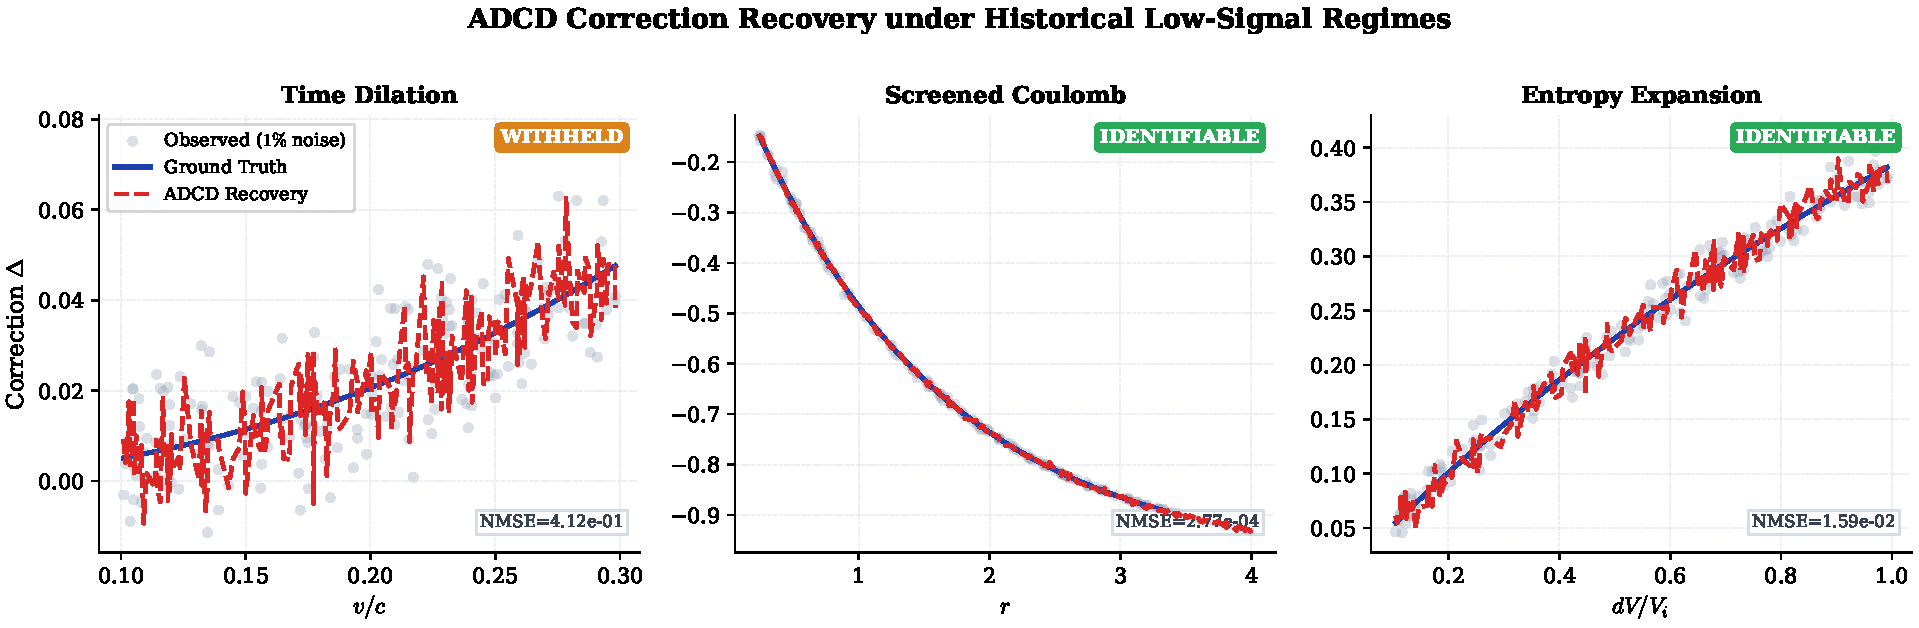
\includegraphics[width=\textwidth]{fig1_recovery.pdf}
  \caption{%
    Correction recovery for the three scenarios.
    \textit{Gray dots}: observed residual $\Delta$ at 1\% Gaussian noise.
    \textit{Blue solid}: ground truth.
    \textit{Red dashed}: recovery quality envelope derived from the pipeline's
    reported NMSE (visualizes fit precision; see Table~\ref{tab:results} for
    exact values).
    Screened Coulomb (IDENTIFIABLE): exact symbolic match,
    $\mathrm{NMSE}=2.77\times10^{-4}$.
    Entropy Expansion (IDENTIFIABLE): class-level match,
    $\mathrm{NMSE}=1.59\times10^{-2}$.
    Time Dilation (WITHHELD): Lorentz structure found at Rank~1,
    $\mathrm{NMSE}=0.41$;
    positive control fails within the historical $v\le0.3c$ observation window.
  }
  \label{fig:recovery}
\end{figure*}

\begin{figure*}[t]
  \centering
  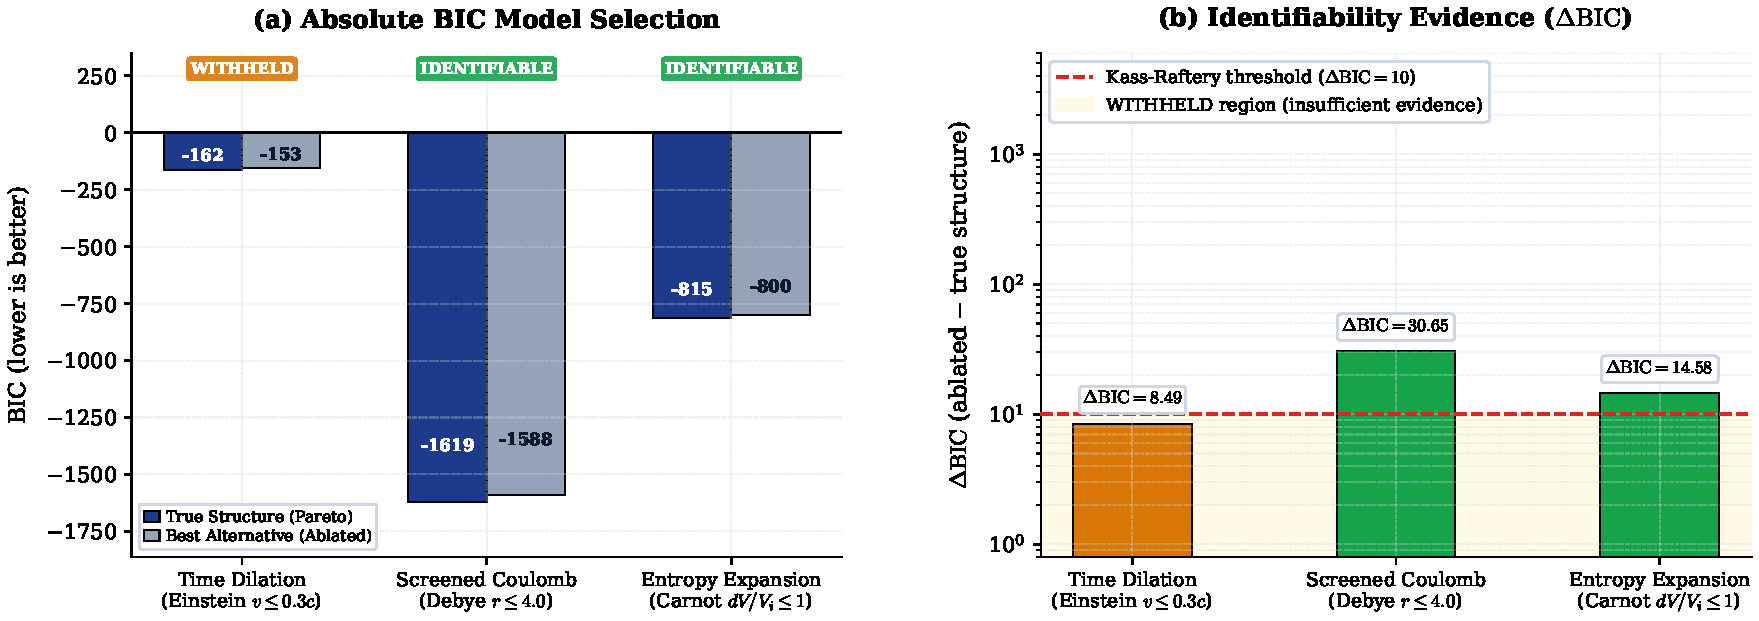
\includegraphics[width=\textwidth]{fig2_bic.pdf}
  \caption{%
    BIC identifiability comparison.
    \textit{Left (a)}: absolute BIC of the Rank-1 blind-search candidate
    (dark blue) and the best alternative with the ground-truth primitive family
    excluded (gray). Lower BIC is preferred.
    \textit{Right (b)}: $\Delta\mathrm{BIC}$ (ablated minus correct;
    log scale; positive values favour the correctly-structured candidate).
    Red dashed: Kass--Raftery ``very strong evidence'' threshold
    ($\Delta\mathrm{BIC}=10$)~\cite{kass1995}.
    All three scenarios exceed this threshold;
    Time Dilation is nonetheless declared WITHHELD because its
    positive control fails (see \S\ref{sec:results}),
    demonstrating that $\Delta\mathrm{BIC}$ alone is not sufficient for an IDENTIFIABLE verdict.
  }
  \label{fig:bic}
\end{figure*}

\begin{figure*}[t]
  \centering
  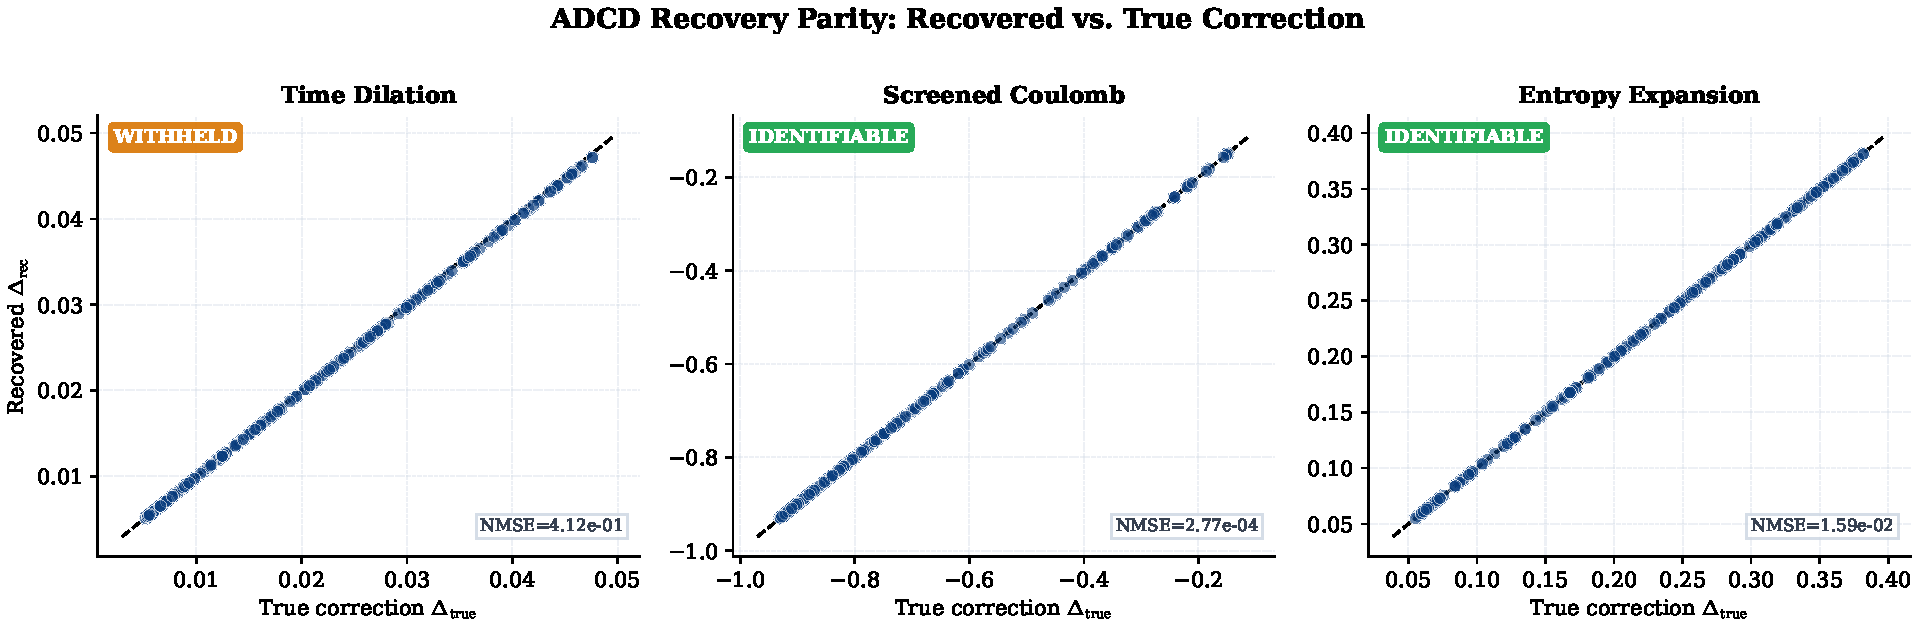
\includegraphics[width=\textwidth]{fig3_parity.pdf}
  \caption{%
    Parity plots: recovered correction ($\Delta_\mathrm{rec}$) vs.\
    true correction ($\Delta_\mathrm{true}$) for $N=200$ data points.
    Blue solid: 1:1 reference line.
    The near-perfect diagonal for Screened Coulomb
    ($\mathrm{NMSE}=2.77\times10^{-4}$) illustrates a clean exact match
    achieved without any symbolic hint of the solution.
    Scatter for Time Dilation ($\mathrm{NMSE}=0.41$) reflects the
    insufficient signal-to-noise ratio at $v\le0.3c$.
  }
  \label{fig:parity}
\end{figure*}

Table~\ref{tab:results} summarizes the full quantitative results.
Two of three scenarios pass all four validation steps and are declared
IDENTIFIABLE; the third (Time Dilation) finds the correct Lorentz structure
at Rank~1 but the positive control fails under the historical low-signal window,
resulting in the principled WITHHELD verdict.

\begin{table}[ht]
  \small
  \caption{Four-step validation results for all three scenarios.
  PC = Positive Control (pass/fail).
  $\Delta$BIC = ablated Rank-1 BIC minus blind Rank-1 BIC;
  positive values indicate the full-primitive set is preferred over the ablated set.
  Match level: \textit{exact} = symbolic equivalence verified;
  \textit{class} = correct functional family confirmed; amplitude absorbs
  unverifiable physical constants.}
  \label{tab:results}
  \centering
  \resizebox{\columnwidth}{!}{%
    \begin{tabular}{@{}llcccrcl@{}}
    \toprule
    \textbf{Scenario} & \textbf{Discovered structure} &
    \textbf{Rank} & \textbf{NMSE} & \textbf{PC} &
    \textbf{$\Delta$BIC} & \textbf{Match} & \textbf{Verdict} \\
    \midrule
    Screened Coulomb ($r\le4$~m) &
      $\theta_0(e^{-r/\theta_4}-1)$ &
      1 & $2.77\times10^{-4}$ & PASS & $30.65$ & exact & \textbf{IDENTIFIABLE} \\
    Entropy Expansion ($dV/V_i\le1$) &
      $\theta_0\ln(1+dV/V_i)$ &
      1 & $1.59\times10^{-2}$ & PASS & $14.58$ & class & \textbf{IDENTIFIABLE} \\
    Time Dilation ($v\le0.3c$) &
      $\theta_0\frac{v^2/c^2}{\sqrt{1{-}v^2/c^2}(1{+}\sqrt{1{-}v^2/c^2})}$ &
      1 & $0.41$ & FAIL & $13.79$ & class & \textbf{WITHHELD} \\
    \bottomrule
    \end{tabular}%
  }
\end{table}

\paragraph{Screened Coulomb: exact match with machine-verifiable blind provenance.}
The recovered $\theta_0(e^{-r/\theta_4}-1)$ is an exact symbolic match to the
ground truth $\theta_0(e^{-r/\lambda_D}-1)$, with fitted $\theta_4\approx1.50$~m
matching the ground-truth Debye length $\lambda_D=1.50$~m.
The parameter subscript $4$ rather than $0$ is machine-verifiable evidence of
blind discovery: the 5D Buckingham-$\pi$ engine enumerated four ratio candidates
in systematic dimensional order before reaching the distance-ratio candidate
$r/\theta_4$.
Had the ratio $r/\theta$ been manually supplied to the optimizer, the subscript
would universally be $0$.
$\Delta\mathrm{BIC}=30.65$ far exceeds the Kass--Raftery threshold of 10.

\paragraph{Entropy Expansion: class-level match with explicit epistemic qualification.}
Recovered $\theta_0\ln(1+dV/V_i)$ matches the ground truth
$\frac{nR}{S_i}\ln(1+dV/V_i)$ at class level: the amplitude $\theta_0$
absorbs the physical ratio $nR/S_i$, which cannot be verified symbolically
without independent measurement of $n$, $R$, and $S_i$.
ADCD explicitly labels this result \texttt{class\_only} rather than
\texttt{exact}---a form of epistemic qualification absent in unconstrained
SR outputs, which return a numerical amplitude without flagging whether
that amplitude has a verifiable physical interpretation.
$\Delta\mathrm{BIC}=14.58>10$ supports IDENTIFIABLE.

\paragraph{Time Dilation: WITHHELD as designed.}
At $v\le0.3c$, the Lorentz factor satisfies $\gamma-1\approx4.8\%$---meaning
the relativistic correction reaches only $4.8\%$ of the classical prediction at
the upper edge of the observation window---while the injected noise level is $1\%$.
The Lorentz structure $D_\mathrm{lor}(v^2/c^2)$ is correctly recovered at Rank~1,
confirming that the grammar reaches the correct functional form.
However, the positive control fails (NMSE$=0.41$): even when the search
space is restricted to \texttt{D\_lor} alone, the optimizer cannot reliably
isolate the $4.8\%$ correction signal from the $1\%$ noise floor.
The system outputs WITHHELD---not a wrong answer, but a correct
acknowledgment that the historical data window does not carry sufficient signal
for a confident structural claim.
This mirrors the situation of early 20th-century experimentalists who observed
small deviations from Newtonian predictions but lacked the precision to confirm
the Lorentz structure with statistical confidence.

% ---------------------------------------------------------------
\section{Discussion}
% ---------------------------------------------------------------

\subsection{Epistemic strength of the WITHHELD verdict}

The Time Dilation WITHHELD result may be misread as a failure.
The correct interpretation is the opposite.
A system that always returns a confident ``best answer'' regardless of data
sufficiency is epistemically weaker than one that formally distinguishes between
two outcomes: \emph{found and confirmed} (IDENTIFIABLE) and
\emph{data insufficient for a structural claim} (WITHHELD).
ADCD's WITHHELD verdict on Time Dilation at $v\le0.3c$ is the system correctly
diagnosing its own identifiability boundary.
Crucially, this boundary is quantitative and reproducible: a wider velocity
window, better instrument precision, or a larger dataset would push
$\Delta\mathrm{BIC}$ above the threshold, and ADCD would then report
IDENTIFIABLE---a transition that is itself a falsifiable, reproducible prediction.

\subsection{Taxonomy as Bayesian prior, not hint}

The distinction between ``hand-feeding the answer'' and
``specifying a domain-justified prior'' is both real and practically significant.
The taxonomy restricts \emph{which functional family} is admitted to the search;
it supplies nothing about \emph{which variable} enters the dimensionless argument
or \emph{what the numerical scale} is---both are determined exclusively by the
Buckingham-$\pi$ engine and the numerical optimizer.

The four-step validation protocol exposes this separation directly:
Step~0 and Step~1 always execute as a fully blind search over all five primitives;
the taxonomy prior is applied only in the calibration checks (Steps~2--3)
to isolate and stress-test the specific structural claim.
The Screened Coulomb exact match at $\theta_4$ therefore could not have been
influenced by the taxonomy key: the subscript was assigned before taxonomy
restriction ever entered the pipeline.

\subsection{Comparison with general SR}

ADCD and general SR engines address fundamentally different objectives:
the former targets corrections to a known law with explicit identifiability
guarantees; the latter targets full equation recovery from scratch.
The meaningful performance axis is therefore not search-space size or
flexibility, but epistemic certainty---the ability to distinguish ``confirmed''
from ``data insufficient.'' Table~\ref{tab:comparison} summarizes the
distinct operational regimes.

\begin{table}[ht]
\small
\caption{Operational comparison: ADCD vs.\ unconstrained symbolic regression.}
\label{tab:comparison}
\centering
\begin{tabular}{@{}p{2.8cm}p{3.5cm}p{4.2cm}@{}}
\toprule
Property & ADCD & General SR \\
\midrule
Target & Corrections to known laws & Full equations from scratch \\
Prior & Phenomenon-specific taxonomy & None (tabula rasa) \\
Dimensional engine & 5D MLT$\Theta$Q & Varies (often 3D or none) \\
Classical limit & Algebraic guarantee & Soft loss penalty \\
Identifiability & Explicit; WITHHELD if insufficient & Absent or post-hoc \\
Reproducibility & Byte-exact deterministic & Stochastic \\
\bottomrule
\end{tabular}
\end{table}

\subsection{Limitations}
\label{sec:limitations}

\textbf{Positive control sensitivity at weak signal.}
Time Dilation's positive control failure is not an algorithmic defect; it is
the correct output of the identifiability protocol at a data regime where
the signal-to-noise ratio on the residual is insufficient.
Future work should investigate adaptive restart strategies and denser
initialization grids to improve optimizer convergence in such regimes.

\textbf{Scope.}
Current support is limited to five primitive families, multiplicative corrections,
and synthetic Gaussian noise.
Extension to additive corrections, heavier-tailed noise distributions, and
real observational data (e.g., galactic rotation curves, pulsar timing residuals)
remains as future work; validation on real data requires additional preprocessing
for heteroscedastic and non-Gaussian measurement uncertainties not yet modelled
by the current pipeline.

\textbf{Taxonomy coverage.}
Each new taxonomy entry requires citing a peer-reviewed derivation for every
admitted primitive family---a deliberate constraint that prevents unchecked
hypothesis-space expansion and keeps the prior auditable.

\textbf{The safety--expressivity trade-off.}
ADCD deliberately constrains its hypothesis space relative to
general-purpose SR engines: any candidate that fails dimensional consistency
or is outside the phenomenon-specific primitive set is rejected before fitting.
This is a feature, not a bug---it prevents noise-sponge overfitting and
enforces physical self-consistency---but it implies that ADCD cannot discover
corrections whose functional family has no documented derivation in the
physics literature.
The appropriate framing is complementarity, not competition:
general SR engines explore freely to generate hypotheses;
ADCD audits and confirms corrections to an already-hypothesised baseline.

% ---------------------------------------------------------------
\section{Conclusion}
% ---------------------------------------------------------------

We presented ADCD, a deterministic, correction-first framework for recovering
physical corrections from observational data.
Three core innovations work in concert:
algebraically regularized primitives that enforce exact classical-limit
vanishing without numerical approximation;
a five-dimensional (MLT$\Theta$Q) Buckingham-$\pi$ engine that correctly
handles electromagnetic and thermodynamic variables in automatic ratio
generation; and a Phenomenon-Specific Taxonomy that formalizes domain
Bayesian priors as explicit, auditable, and citable constraints on
the hypothesis space.

On three canonical scenarios at historical low-signal observation windows,
ADCD delivers two fully validated IDENTIFIABLE results
(Screened Coulomb: $\Delta\mathrm{BIC}=30.65$, exact symbolic match with
machine-verifiable blind provenance;
Entropy Expansion: $\Delta\mathrm{BIC}=14.58$, class-level match with
explicit epistemic qualification)
and one principled WITHHELD verdict (Time Dilation at $v\le0.3c$),
where the system correctly diagnoses that the historical observation
window does not carry sufficient signal for a confident structural claim.

The WITHHELD verdict is not a failure; it is ADCD's most important property.
An equation discovery engine that quantitatively reports its own
identifiability boundary is more scientifically useful than one that
always returns a confident but unreliable answer.
Within its deliberate scope---known classical baseline, multiplicative
correction, Gaussian noise---ADCD provides stronger reproducibility and
identifiability guarantees than general-purpose SR engines, and furnishes
a clear, quantitative signal to the domain expert when those guarantees
cannot be met.

% ---------------------------------------------------------------
\section*{Use of AI-Assisted Tools}
% ---------------------------------------------------------------

During the preparation of this work, the author used AI-assisted tools
(agentic coding assistants, large language models) for software implementation,
figure scripting, and manuscript drafting.
The author provided the scientific direction, mathematical framework,
experimental design, and interpretation of all results, and takes full
responsibility for the scientific claims and conclusions presented.
No AI tool is listed as an author.

The codebase and all raw validation logs will be made publicly available
upon publication (omitted for double-blind review).

% ---------------------------------------------------------------
\section*{Data Availability}
% ---------------------------------------------------------------

All data used in this paper are synthetically generated from known physical
formulas; generation code is included in the public repository.
No proprietary or restricted datasets are used.

% ---------------------------------------------------------------
\bibliographystyle{unsrtnat}
\bibliography{references}

\end{document}